\documentclass[11pt]{article}
\usepackage{icmlko}
\begin{document}

\title{판이 못 보는 0.39 --- 표지를 무엇으로 만드느냐가 전이의 전부다}
\author{월드모델 실험실}
\date{노트 423 · 2026년 8월 3일}
\maketitle

\begin{abstract}
노트 420·421·422가 같은 물음을 세 번 틀리게 풀었다 --- \emph{왜 도메인
표지는 하나여야 하나.} 칸 수 때문(420)도, 나무가 둘을 곱해서(421)도
아니었고, 곱을 막으니 더 나빠져서(422) ``관측으로 둔다''로 닫았다.

물음이 틀렸다. 안 재 본 팔이 하나 있었다 --- \textbf{grp2 하나만}.
구조도 눈금 규칙도 같고 \textbf{field 만 다르다}.

\begin{center}
\begin{tabular}{lrrr}
\hline
표지 & 덮음 & 판 & KR 만화 전이 \\
\hline
\texttt{grp} 하나 & 7 & $+0.4723$ & $\mathbf{+0.1970}$ \\
\texttt{grp2} 하나 & 8 & $+0.4718$ & $\mathbf{-0.1918}$ \\
\hline
\end{tabular}
\end{center}

같은 유보 행 짝 되뽑기로 차 $+0.3901$, 95\% $[+0.2886, +0.4898]$,
$1000/1000$. \textbf{전이가 $+0.20$ 에서 $-0.19$ 로 뒤집힌다.} 그런데
\textbf{판은 $0.0005$ 밖에 안 다르다.}

\textbf{개수가 아니라 재료였다.} 그리고 세 노트의 수수께끼가 한꺼번에 풀린다.
\end{abstract}

\section{네 값이 한 줄로 선다}

\begin{center}
\begin{tabular}{lr}
\hline
 & KR 전이 \\
\hline
\texttt{grp} 만 (좋은 표지) & $+0.1970$ \\
\texttt{grp}$+$\texttt{grp2} (나무가 고를 수 있음) & $+0.0819$ \\
SplitBag (반반 강제) & $+0.0064$ \\
\texttt{grp2} 만 (나쁜 표지) & $-0.1918$ \\
\hline
\end{tabular}
\end{center}

두 팔의 \textbf{평균}은 $(+0.1970 - 0.1918)/2 = +0.0026$ 이다. SplitBag 은
자루 절반씩을 강제로 섞은 것이니 평균이 나와야 하는데 --- \textbf{실측
$+0.0064$} 다. 예측과 실측이 맞는다.

둘 다 보이는 팔($+0.0819$)이 평균보다 높은 것도 맞물린다 --- 나무가 둘을
다 보면 \textbf{좋은 쪽에 더 기댈 수 있다.} 순서가 전부 설명된다.

\textbf{노트 422의 ``표지는 하나만''은 틀렸다.} 표지가 둘이어서 나빴던 게
아니라 \textbf{둘 중 하나가 나빴다.}

\section{판은 이 차이를 못 본다}

이것이 이 노트에서 제일 무거운 줄이다. 두 표지의 판 차는 $0.0005$ --- 씨앗
잡음($\pm 0.0007$)보다 작다. \textbf{판으로는 둘을 못 고른다.} 그런데 목표
쪽에서는 $0.39$, 부호가 뒤집히는 차다.

포트폴리오의 순위(유보 표본의 판 $\rho$)는 \textbf{이 축에서 눈이 멀어
있다.} 노트 420이 규약을 하나 더한 것($전이를 확실히 잃는 변경은 판이
통과해도 안 넣는다$)이 여기서 값을 한다 --- 그 규약이 없었으면
\texttt{grp2} 를 판만 보고 갈아 끼웠을 수 있고, 판은 그대로인 채 전이가
$+0.20 \to -0.19$ 로 뒤집혔을 것이다.

\section{무엇이 두 무리를 가르나}

\begin{center}
\begin{tabular}{lll}
\hline
도메인 & \texttt{grp} $(+0.197)$ & \texttt{grp2} $(-0.192)$ \\
\hline
웹툰 & 연령 유형 & 데일리패스 \\
모바일 & 무료 여부 & 심의 등급 \\
애니 & 매체 & 오리지널 여부 \\
세계애니 & 포맷 & 원작 매체 \\
게임 & 무료 여부 & 플랫폼 수 \\
펀딩 & 카테고리 & 성인 전용 \\
도서 & 출판사 & 판형 \\
\hline
\end{tabular}
\end{center}

눈으로 보면 왼쪽은 \textbf{무엇인가}(매체 · 포맷 · 카테고리 · 출판사)에
가깝고 오른쪽은 \textbf{어떻게 파는가}(데일리패스 · 심의 · 플랫폼 수 ·
판형)에 가깝다. \textbf{그럴듯하지만 $n{=}7$ 짜리 눈짐작이다} --- 노트 401이
같은 자리에서 속았으므로 여기서는 \textbf{짓지 않는다.} 다음 사이클의
사전 등록 후보로만 적는다.

\section{남은 것}

\begin{tabular}{lp{7.0cm}}
\hline
자리마다 하나씩 & 일곱 자리를 하나씩 grp2 쪽으로 바꿔 가며 재면 \textbf{어느
자리가 부호를 뒤집는지} 나온다. 전이를 더 살 여지가 거기 있다 \\
``무엇인가 대 어떻게 파는가'' & 위 눈짐작을 사전 등록해서 재는 것 \\
판의 눈먼 축 & 판이 $0.0005$ 로 못 가르는 선택이 목표를 $0.39$ 움직인다.
\textbf{순위 지표를 하나 더 두어야 하나} --- 노트 419가 열어 둔 물음 \\
\hline
\end{tabular}

\begin{figure}[h]
\centering
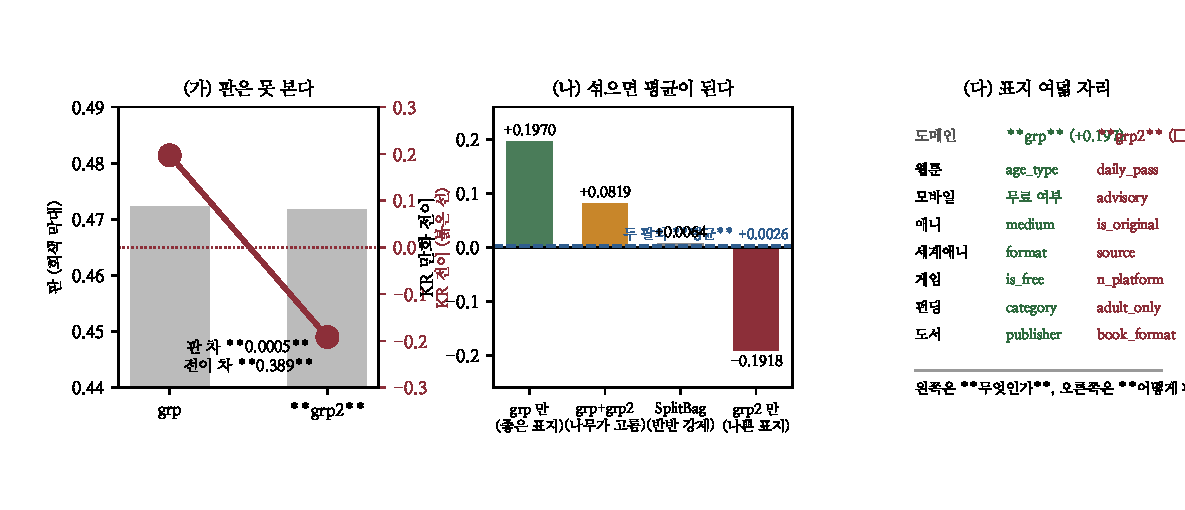
\includegraphics[width=\textwidth]{figs/fig423.pdf}
\caption{(가) 판은 $0.0005$, 전이는 $0.389$. (나) 네 팔이 한 줄로 서고
SplitBag 이 두 팔의 평균에 앉는다. (다) 표지 여덟 자리.}
\end{figure}

\end{document}
